\documentclass[pss]{wiley2sp} % provides pss two-column style
\usepackage{amsmath}
\usepackage{soul}
%\usepackage{bm}              % uncomment these two packages if you
%\usepackage{w-greek}         % need extended greek-letter functionality in math mode

\graphicspath{{figures/}{./}}

\renewcommand{\arraystretch}{1.2} % please do not remove or change
\tolerance=400
\emergencystretch=10pt


\begin{document}

% Title of the article
\title{\emph{Ab initio} calculation of the depth-dependent optical reflectance
from layer-by-layer atomic disorder}

% Abbreviated title for the page headers
\titlerunning{Calculation of the depth-dependent optical reflectance}

% Authors
\author{%
  Sean M. Anderson\textsuperscript{\textsf{\bfseries 1}},
  Bernardo S. Mendoza\textsuperscript{\Ast,\textsf{\bfseries 1}},
  Ram\'on Carriles\textsuperscript{\textsf{\bfseries 1}}
}

% Abbreviated list of authors for the page headers
\authorrunning{Anderson et al.}

%E-mail-address of corresponding author
\mail{e-mail
  \textsf{bms@cio.mx}, Phone:
  +52-477-4414200, Fax: +52-477-4414209}

% author's affiliations/addresses
\institute{%
  \textsuperscript{1}\,Centro de Investigaciones en \'Optica, A.C.,
                       Le\'on, Guanajuato 37150, Mexico}

\received{XXXX, revised XXXX, accepted XXXX} % do not change, will be filled in by the publisher
\published{XXXX} % do not change, will be filled in by the publisher

% Please select about four verbal keywords for your manuscript.
\keywords{reflectance spectroscopy, atomic disorder, CAP, surface, strain}

\abstract{
\abstcol{We present a simple model to study the effects of displacing a single 
atomic monolayer on the linear optical properties of a material. As an example,
we calculate the change in reflectance of a Si(111)(1$\times$1):H slab after
disordering successively deeper atomic layers. We find that the reflectance
varies significantly at photon energies above 2.0\,eV, and that the disordered
slab produces a larger reflectance than the relaxed slab.}
{The results also show a quantitative difference in the contribution from the
odd and even atomic layers to the calculated reflectance. This simplified model
is a first approach; also, it can be extended to consider more realistic systems
that can be probed by techniques such as coherent acoustic phonon (CAP)
spectroscopy, and can also be applied to two-dimensional materials.}
}

\maketitle   % please do not remove

%%%%%%%%%%%%%%%%%%%%%%%%%%%%%%%%%%%%%%%%%%%%%%%%%%%%%%%%%%%%%%%%%%%%%%%%%%%%%%%
%%%%%%%%%%%%%%%%%%%%%%%%%%%%%%%%%%%%%%%%%%%%%%%%%%%%%%%%%%%%%%%%%%%%%%%%%%%%%%%

\section{Introduction}\label{sec:intro}

The characterization and profiling of inhomogeneities in solid state materials
has become increasingly important for the development of new and improved
optoelectronic technologies. This includes, but is not restricted to, studying
the effects of defects or impurities on the local optical properties of the host
materials, as well as determining specific defect profiles. While some of the
existing techniques are destructive, optical methods are non-invasive and
usually work in situ; thus, it is desirable to develop these tools in order to
better analyze the optical response of a given material. These experimental
studies should be coupled with the necessary theoretical framework to support
the observations. Namely, \emph{ab initio} calculations can yield
frequency-dependent optical functions that take into account any lattice
disorder, strain, inhomogeneities or defects that may be present. The
calculation of the linear optical properties from both surface and bulk regions
%%
\cite{hoganPRB98,palummoPRB99,hoganPRB03,mendozaPRB06,palummoPRB09,tancognePRB14,tancognePRB15}
%%
is now computationally efficient and numerically more accurate than the
traditional phenomenological or Maxwell models often found in the literature.
This enables an in-depth profiling of the interactions between structural
characteristics and the local optoelectronic properties of a given material.

To this end, we have developed a simple model to study the effects of atomic
disordering in a sample surface-bulk system. In this model, we move the
$z$-coordinate for each individual atom, one at a time, away from the
equilibrium position in small, uniform translations, starting from the surface
layer down into the bulk. {\color{red}Since the unit cell is repeated along the
$xy$ plane, this is equivalent to translating individual monolayers within the
structure.} The linear optical response function can then be
calculated for the entire structure, taking into account the newly disordered
atomic positions. Although this proposed model is an oversimplification of the
real physical response of the material, it is a first building block for more
sophisticated theoretical treatments. In particular, once the individual
monolayer responses to the lattice deformations are known, it should be possible
to calculate the induced strain response for a specific slab or surface. The
generated strain need not be uniform, as it could also be any arbitrary material
deformation induced by a traveling wave or another excitation, such as the one
induced in a coherent acoustic phonon (CAP) experiment.

CAP spectroscopy (also called picosecond ultrasonics) is an acousto-optical
technique that is well suited for these kinds of measurements. It is a
pump-probe technique
\cite{thomsenPRL84,thomsenPRB86,grahnJQE89,linJAP91,pfeiferPRL92} that involves
an ultrafast, high-intensity \emph{pump} pulse impinging on an absorbing
material, and a second \emph{probe} pulse that senses changes in the optical
properties of the material that are induced by the pump pulse. The pump pulse is
absorbed at the surface, establishing a transient strain wave at the sample
surface that traverses the material as a longitudinal acoustic phonon. This CAP
wave acts as a localized strained layer that moves down into the material at the
material-specific phonon velocity. It modifies the local dielectric constants,
creates discontinuities, and causes a periodic modulation of the optical
properties. The CAP wave effectively samples different layers as it travels
through the material, which positions it as a promising noninvasive option for
measuring optical properties as a function of depth and across material
interfaces, as well as being sensitive to lattice deformation and
inhomogeneities. In particular, the technique has been extensively used to study
the structural properties of metals \cite{rossignolPRL05,parkPRB05},
semiconductors
%%
\cite{wuAPL06,matsudaPRL04,millerPRB06,wenAPL07,xuPSSC08,babilottePRB10,hudertJAP08},
%%
and transition metal oxysalts
\cite{limAPL03,bozovicPRB04,ruelloPRB09,ruelloAPL12,chenAPL12}. Likewise, it has
been shown to be an effective tool for determining thin film thicknesses
\cite{gusevJAP11,matsudaJOSAB02}, elasto-mechanical
\cite{grahnAPL88a,grahnAPL88b,rossignolPRL05,taneiPRL08} and optical properties
\cite{qiPRB10,millerPRB06,xuPSSC08}, low-frequency phonon dispersion and
attenuation mechanisms \cite{zhuPRB91,dalyPRB09}, buried interface roughness
\cite{tasAPL98}, inhomogeneities in disordered films \cite{gusevJAP11}, doping
profiles \cite{hudertJAP08}, lattice defects
\cite{steigerwaldJAP12,steigerwaldAPL09,gregoryAPL12,baydinAPLP16}, and shear
strain waves using time-resolved polarization measurements
\cite{mounierEPJST08,mounierOE10}.

Our model could help in the understanding of the experiments based on techniques
such as CAP or reflectance anisotropy spectroscopy (RAS). There are some
available \emph{ab initio} calculations applied towards studying CAP
spectroscopy \cite{lawlerMRE14,steigerwaldJAP12}, but we consider that there is
room for more theoretical development in this area. Accordingly, we have
developed our model with some of the basic characteristics from these types of
experiments. The inter-atomic displacements that we consider in our model (up to
0.224\,{\AA}) are of the same order as those induced in real samples during a
CAP experiment \cite{lawlerMRE14}. The spatial resolution of CAP is on the order
of 100\,{\AA} \cite{thomsenPRB86}, while RAS can probe only a few monolayers on
the surface, and current \emph{ab initio} methods are very well suited for
analysis at this scale \cite{andersonPRB16b,andersonFMATS17}. These
considerations result in calculated reflectivity changes (described in Sec.
\ref{sec:results}) that are within the detection sensitivity range accessible
with lock-in techniques \cite{gregoryAPL12}. We consider that our model  manages
to yield relevant insight about strain waves in surface-bulk systems, and helps
elucidate the physical phenomena dictating the observed changes in reflectance.
Additionally, our model can be easily applied towards the study of
two-dimensional materials, which have very promising optoelectronic properties.

This paper is organized as follows. In Sec. \ref{sec:theory}, we present the
relevant equations and theory that describe the calculation of the linear
optical response and the reflectance difference spectrum. In Sec.
\ref{sec:results}, we present and analyze the calculated reflectance using the
Si(111)(1$\times$1):H surface as a test case. Finally, we list our conclusions
and final remarks in Sec. \ref{sec:conc}.

%%%%%%%%%%%%%%%%%%%%%%%%%%%%%%%%%%%%%%%%%%%%%%%%%%%%%%%%%%%%%%%%%%%%%%%%%%%%%%%
%%%%%%%%%%%%%%%%%%%%%%%%%%%%%%%%%%%%%%%%%%%%%%%%%%%%%%%%%%%%%%%%%%%%%%%%%%%%%%%

\section{Theory}\label{sec:theory}

To model a semi-infinite crystal, we utilize a slab, consisting of $N$ atomic
layers and thickness $D$ inside a supercell of total height $L$, that includes
the vacuum region required when using the repeated slab scheme, and is large
enough to avoid the wave function tunneling to neighboring supercells
\cite{mendozaPRB06}. The surface is parallel to the $xy$ plane, with the surface
normal in the $z>0$ direction. Following Ref. \cite{mendozaPRB06}, the
reflectance difference spectrum $\Delta R$ is defined as
\begin{equation}\label{eq:1}
\Delta R 
= \frac{R_{x}+R_{y}}{2}\bigg|_{\mathrm{relaxed}}
- \frac{R_{x}+R_{y}}{2}\bigg|_{\mathrm{perturbed}}
,
\end{equation}
where $R_{\mathrm{a}}$ ($\mathrm{a} = x$ or $y$) is the normal incident
reflectance for linearly polarized light in the $\hat{\mathbf{a}}$ direction. As
explained in the introduction, our idea is to move the atoms of the slab away
from their equilibrium positions, calculate $R_{\mathrm{a}}$ for this perturbed
slab, and study the difference with the value of the unperturbed or relaxed
structure via $\Delta R$. $R_{\mathrm{a}}$ can be calculated through the optical
response of the slab system \cite{delsolechap95} as
\begin{equation}\label{eq:2}
R_{\mathrm{a}} = 
4\left(\frac{\omega}{c}\right)
\mathrm{Im}
\bigg[
\frac{(D/2)\chi^{\mathrm{aa}}_{sc}(\omega)}
     {\boldsymbol{\chi}^{~}_{b}(\omega)}
\bigg]
,
\end{equation}
where $\omega$ is the angular frequency of the normally incident light impinging
from the vacuum side, $c$ is the speed of light, $D/2$ is the half-slab
thickness, $\boldsymbol{\chi}_{sc}(\omega)$ is the linear susceptibility for the
supercell system, and $\boldsymbol{\chi}^{~}_{b}(\omega)$ is the linear
susceptibility of the isotropic bulk crystal.

Within the usual independent-particle framework \cite{tancognePRB14}, we have
that
\begin{equation}\label{eq:3}
\begin{split}
\chi^{\mathrm{aa}}(\omega) 
& = \frac{e^{2}}{\hbar}
  \int \frac{d\mathbf{k}}{8\pi^3}
  \sum_{vc} \frac{1}{\omega_{cv}(\mathbf{k})}
  \mathrm{Im}
  \Big[
    v^{\mathrm{a}}_{cv}(\mathbf{k})r^{\mathrm{a}}_{vc}(\mathbf{k})
  \Big] \\
& \times
  \Bigg(
      \frac{1}{\omega_{cv}(\mathbf{k})-\omega-i\eta}
    + \frac{1}{\omega_{cv}(\mathbf{k})+\omega+i\eta}
\Bigg) 
,
\end{split}
\end{equation}
with $\hbar \omega_{n}(\mathbf{k})$ being the energy of the electronic band $n$
at point $\mathbf{k}$ in the irreducible Brillouin zone,
$\omega_{nm}(\mathbf{k}) = \omega_{n}(\mathbf{k}) - \omega_{m}(\mathbf{k})$;
$n,m = v$ corresponds to a valence band, and $n,m = c$ is a conduction band.
Here, $\mathbf{v}_{nm}(\mathbf{k})$ and $\mathbf{r}_{nm}(\mathbf{k})$ are the
matrix elements of the electron velocity and position operators, with
$\mathrm{a} = x$ or $y$. Lastly, $\eta$ can be used to include the broadening of
the electronic levels. {\color{red}Many-body interactions can be included in an approximate
manner using a scissors operator approach in Eq. \eqref{eq:3}, following Ref.}
\cite{andersonPRB15}. In this way, we adjust the calculated energy band gap to
the correct experimental value. In Eq. \eqref{eq:3}, the first energy
denominator includes the \emph{resonant} terms, while the second denominator
includes the \emph{nonresonant} terms. Indeed, by taking $\eta\to 0$, we obtain
Dirac delta functions $\delta(\omega_{cv}(\mathbf{k}) - \omega)$ for the
resonant term, and $\delta(\omega_{cv}(\mathbf{k}) + \omega)$ for the
nonresonant term. For positive energies, only the resonant term will contribute
to $\chi^{\mathrm{aa}}(\omega)$, whereas the nonresonant term will yield zero
contribution. As shown in Ref. \cite{tancognePRB14}, both terms are needed to
accurately calculate $\chi^{\mathrm{aa}}(\omega)$. The bulk susceptibility,
$\boldsymbol{\chi}^{~}_{b}(\omega)$, is obtained by using a bulk unit cell in
Eq. \eqref{eq:3}; likewise, $\boldsymbol{\chi}_{sc}(\omega)$ is obtained by
using a supercell, where it must be properly normalized with respect to the
vacuum included in the total supercell height $L$ \cite{tancognePRB15}. Then, we
take $\boldsymbol{\chi}_{sc}(\omega)\to(L/D)\boldsymbol{\chi}_{sc}(\omega)$, so
that even if a larger vacuum region is included, the results remains invariant.

%%%%%%%%%%%%%%%%%%%%%%%%%%%%%%%%%%%%%%%%%%%%%%%%%%%%%%%%%%%%%%%%%%%%%%%%%%%%%%%
%%%%%%%%%%%%%%%%%%%%%%%%%%%%%%%%%%%%%%%%%%%%%%%%%%%%%%%%%%%%%%%%%%%%%%%%%%%%%%%

\section{Results}\label{sec:results}

We chose the Si(111)(1$\times$1):H surface as a representative test case for our
model. The ideal Si(111) bulk terminated surface has an unsaturated dangling
bond at each of its surface Si atoms; the addition of an H atom at each surface
will passivate this bond and yield an unreconstructed surface with a 1$\times$1
unit cell. In this example, this surface is represented by a centrosymmetric
slab of 38 atoms comprised of 36 Si atoms between one H atom on each surface;
Fig. \ref{fig:3dstruc} presents a graphical representation of this slab. The
hexagonal symmetry of this surface is such that $\chi^{xx}_{sc}(\omega) =
\chi^{yy}_{sc}(\omega)$, and so, $R_{x} = R_{y}$. Choosing a centrosymmetric
slab allows us to carry out the analysis over only half of the slab, since the
other half yields identical results. The self-consistent ground state and the
Kohn-Sham states needed in Eq. \eqref{eq:3}, along with the atomic positions for
the relaxed slab, were calculated in the DFT-LDA framework using the plane-wave
ABINIT code \cite{gonzeCPS09,abinit}. See Ref. \cite{andersonPRB16b} for a
detailed account of this calculation. We found converged results for the surface
$\boldsymbol{\chi}_{sc}(\omega)$ calculation using 244 $\mathbf{k}$ points and a
cutoff energy of 7 Ha; 3107 $\mathbf{k}$ points and a cutoff energy of 10 Ha
were used for the bulk $\boldsymbol{\chi}^{~}_{b}(\omega)$ calculation.
{\color{red} A scissors shift of 0.7 eV was used for the surface, obtained from
$G_{0}W_{0}$ calculations \cite{liPRB10}. For the bulk, we applied a scissors
shift of 0.98 eV in order to adjust the calculated direct band gap to the
experimental value \cite{landolt}.}

To identify which atom will be displaced, we tag each one in consecutive order
starting at the surface, i.e. H$_{1}$ and Si$_{2}$ down to Si$_{19}$ (see Fig.
\ref{fig:3dstruc}). We can see that the odd Si atoms have the vertical bonds
going down and the slanted bonds going up, and vice versa for the even Si atoms.
We displace any given atom \emph{up} (towards $z > 0$) or \emph{down} (towards
$z < 0$) by a percentage $p$ of the $z$ distance between atoms Si$_{2}$ and
Si$_{3}$, which is 0.784\,\AA. {\color{red}We perturb only a single atomic monolayer at a time} from
its equilibrium position; all other atoms remain at their original (relaxed)
positions. We restrict the present study to photon energies that are in the
visible range; the experiments are much easier to perform, and there is no
absorption of light as Im[$\boldsymbol{\chi}_{(sc,b)}(\omega) = 0$] in this
range, since the direct band gap energies, besides being very similar for
surface and bulk, are around 3.05--3.4\,eV
\cite{landolt,ortegaPRB93,brunevalPRB06,liPRB10}.

\begin{figure}[t]%
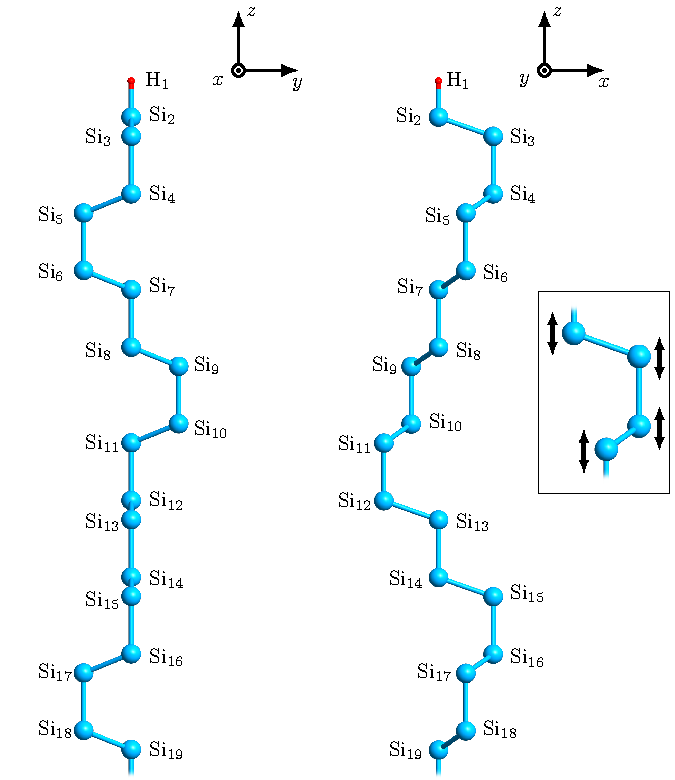
\includegraphics[width=\linewidth]{fig01}
\caption{$xz$ and $yz$ plane views of the relaxed Si(111)(1$\times$1):H
half-slab used in this work. All atoms (balls) are tagged according to their $z$
position within the slab. Each atom is connected to another via vertical or
slanted bonds, represented by interconnecting rods. The inset to the right
depicts the $z$ displacement that was carried out on {\color{red}each atom (and the corresponding monolayer)}, one
at a time.}
\label{fig:3dstruc}
\end{figure}

In Fig. \ref{fig:2}, we present $\Delta R$ vs. $\hbar\omega$ for a $p = 30\%$
(0.224\,\AA) \emph{up} or \emph{down} displacement of selected Si$_{n}$ atoms.
From the plot, we can see that $\Delta R \sim 0$ for energies below 2.0\,eV;
above this value, $\Delta R$ goes monotonically to more negative values, which
implies that the perturbed structure reflects more light than the relaxed
structure. We can also appreciate how the $\Delta R$ spectra can be grouped into
the odd and even displaced Si$_{n}$ atoms. For the even Si$_{2n}$ atoms,
$|\Delta R|$ is larger (smaller) than for the odd Si$_{2n+1}$ atoms, for
\emph{up} (\emph{down}) displacements.

From this grouping, we can observe the influence of the vertical and slanted
bonds on $\Delta R$. When displacing each atom in the \emph{up} direction, the
vertical bonds on the even (odd) Si atoms are compressed (elongated) while the
slanted bond is elongated (compressed), and vice versa for the \emph{down}
displacement. This trend for $\Delta R$ reverses between the \emph{up} and
\emph{down} displacements, and the even and odd Si atoms; thus, displacing an
even atom \emph{down} is similar to displacing an odd atom \emph{up} and vice
versa. This behavior is consistent with the fact that the bond geometry is
reversed from one case to the other; however, the surface breaks the symmetry
along $z$, creating quantitative differences in $\Delta R$. Note that for normal
incidence, the slanted bonds yield a significantly larger contribution to the
linear optical properties over the vertical bonds.

\begin{figure}[b]
\begin{center}
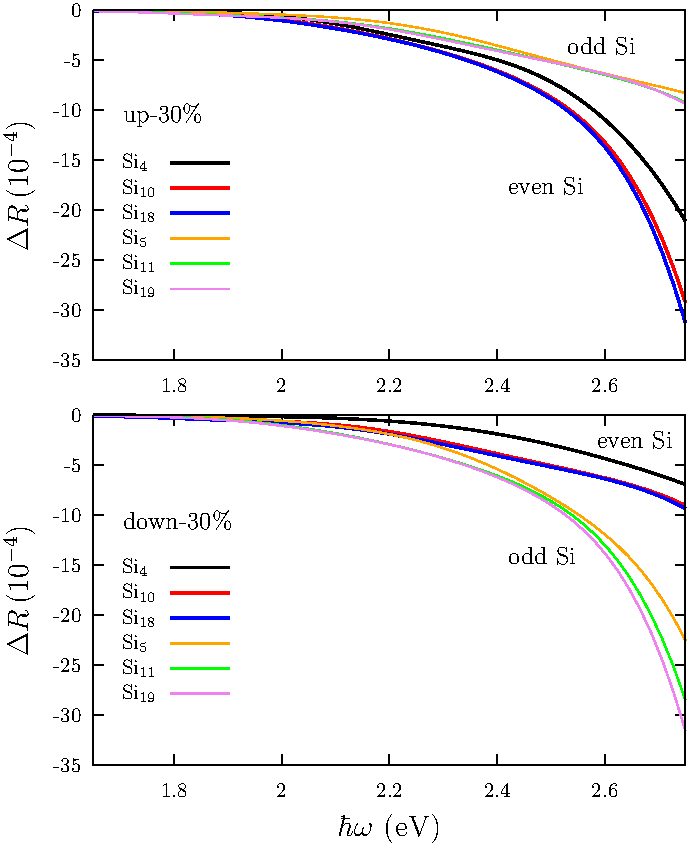
\includegraphics[width=0.9\linewidth]{fig02}
\caption{$\Delta R$ vs. $\hbar\omega$ for a $p = 30\%$ (0.224\,\AA) \emph{up} or
\emph{down} displacement of selected even and odd Si atoms.}
\label{fig:2}
\end{center}
\end{figure}

To proceed with the analysis, in Fig. \ref{fig:3} we plot $\Delta R$ vs. atom
position for a fixed energy of $\hbar\omega = 2.6$\,eV, for values of $p$
between 5--30\% in steps of 5\%, which is equivalent to displacements between
0.040--0.224\,\AA~ in increments of 0.040\,\AA. In Fig. \ref{fig:odd_down}, we
present the odd (H$_{1}$, Si$_{2n+1}$) atoms displaced \emph{down}. For $p =
5\%$, $\Delta R$ remains identical for every atom displacement. As $p$
increases, $\Delta R$ becomes increasingly negative, indicating again that the
perturbed surface has a higher reflectance than the relaxed surface. $\Delta R$
is always zero for H$_{1}$ displacements, which is expected from the fact that
the H atom quenches the surface states, making it optically inactive. It is
interesting to note that as atoms that are farther away from the surface are
displaced, $\Delta R$ reaches a constant value; as the displacement ($p$)
increases, it takes deeper displacements to reach that value. This indicates
that displaced atoms closer to the surface can be discerned by the changes in
$\Delta R$, while displacements occurring towards the bulk of the material would
be difficult to identify individually. In turn, this could be explained from the
fact that the atoms located beyond the influence of the surface will all have
the same effect on $\Delta R$, regardless of their exact depth within the bulk
of the material. In Fig. \ref{fig:even_up}, we present $\Delta R$ for the same
values of $p$ for even (Si$_{2n}$) atoms, displaced \emph{up}. As discussed
above in connection with Fig. \ref{fig:2}, this \emph{up} displacement of the
even atoms is similar to the \emph{down} displacement of the odd atoms; thus,
the qualitative similarities between the results in Figs. \ref{fig:odd_down} and
\ref{fig:even_up} further confirm this fact. Likewise, we present \emph{up}
displacements for the odd atoms in Fig. \ref{fig:odd_up}, and \emph{down}
displacements for the even atoms in Fig. \ref{fig:even_down}. The qualitative
description of these results is similar to our comments above concerning Figs.
\ref{fig:odd_down} and \ref{fig:even_up}. However, we find that $\Delta R$ is
about half the value presented in those figures, which is again in agreement
with Fig. \ref{fig:2}. In summary, we find that $\Delta R$ for atoms displaced
\emph{down} is larger for odd (Si$_{2n+1}$) atoms than for even (Si$_{2n}$)
atoms, as shown in Figs. \ref{fig:odd_down} and \ref{fig:even_down}. Likewise,
we also find that displacing the even atoms \emph{up} produces a larger $\Delta
R$ than the odd atoms, as can be seen from Figs. \ref{fig:even_up} and
\ref{fig:odd_up}.

\begin{figure*}[htb]%
\centering
% \captionsetup{position=above,justification=centering}
\subfloat[Odd atomic layers, displaced \emph{down}.\label{fig:odd_down}]{%
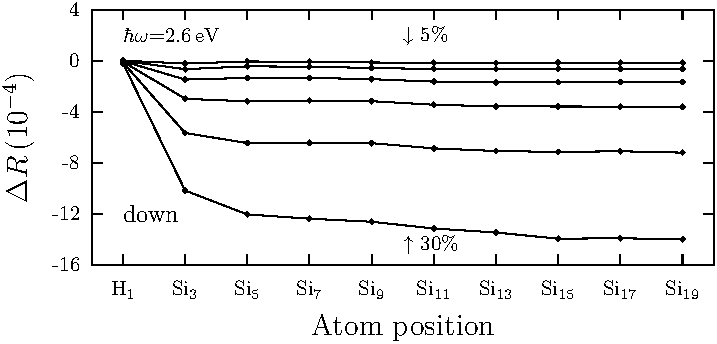
\includegraphics[width=0.47\textwidth]{fig03a}}
\hfill
\subfloat[Even atomic layers, displaced \emph{up}.\label{fig:even_up}]{%
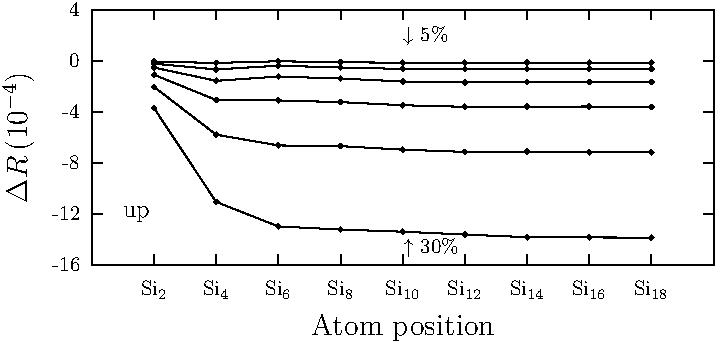
\includegraphics[width=0.47\textwidth]{fig03b}}
\\
\subfloat[Odd atomic layers, displaced \emph{up}.\label{fig:odd_up}]{%
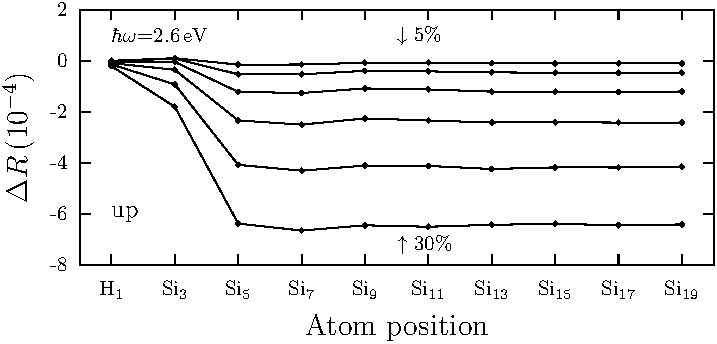
\includegraphics[width=0.47\textwidth]{fig03c}}
\hfill
\subfloat[Even atomic layers, displaced \emph{down}.\label{fig:even_down}]{%
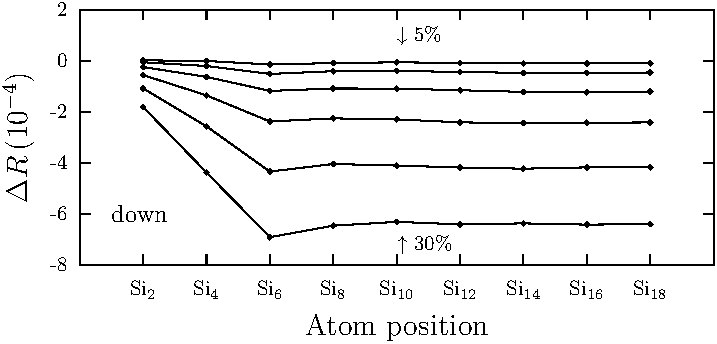
\includegraphics[width=0.47\textwidth]{fig03d}}
%%
\caption{$\Delta R$ vs. atom position (black dots) at $\hbar\omega = 2.6$\,eV,
for values of $p$ between 5--30\% in steps of 5\%. Solid lines are for ease of
viewing. Panel \subref{fig:odd_down}: odd (H$_{1}$, Si$_{2n+1}$) atoms displaced
\emph{down}. Panel \subref{fig:even_up}: even (Si$_{2n}$) atoms displaced
\emph{up}. Panel \subref{fig:odd_up}: odd (H$_{1}$, Si$_{2n+1}$) atoms displaced
\emph{up}. Panel \subref{fig:even_down}: even (Si$_{2n}$) atoms displaced
\emph{down}.}
\label{fig:3}
\end{figure*}

Lastly, in Fig. \ref{fig:4} we show $\Delta R$ vs. the atom position for
different values of $\hbar\omega$, for a $p = 30\%$ \emph{down} displacement
only. The top panel shows the odd (H$_{1}$, Si$_{2n+1}$) atoms, while the bottom
panel shows the even (Si$_{2n}$) atoms. Again, we see lower values for $\Delta
R$ produced by displacing the even atoms than by displacing the odd atoms.
$\Delta R$ remains zero for $\hbar\omega=1.8$\, eV, but as $\hbar\omega$
increases, $\Delta R$ grows increasingly negative; as before, this is in
accordance with the results discussed in Fig. \ref{fig:2}. We note that
equivalent results were obtained for the \emph{up} displacement as a function of
$\hbar\omega$, but are not included here. Most importantly, Fig. \ref{fig:4}
shows conclusive evidence that changes in $\Delta R$ can be used to monitor
vertical displacements of atoms close to the surface, particularly at higher
energies in the visible range.

We propose the following explanation for the calculated changes in reflectance.
For an \emph{up} (\emph{down}) displacement, the even (odd) atoms will have
elongated slanted bonds; for an \emph{up} (\emph{down}) displacement, the odd
(even) atoms will have compressed slanted bonds. If we consider the response of
the bonds as linear harmonic oscillators, an electron in an elongated bond will
have a looser confinement compared to that in a compressed bond. This means that
the electron potential for the elongated (compressed) bond has a lower (higher)
curvature as compared to that of the relaxed bond, implying that the resonant
frequency, being proportional to the curvature, is lower (higher) than for the
relaxed bond. Therefore, the elongated (compressed) bond has a higher (lower)
polarizability, which leads to a {\color{red}larger (smaller) increase in the reflectance.}

Overall, our simple model for layer-by-layer atomic disordering verifies that
detectable changes on the order of $10^{-4}$ occur to $\Delta R$, even when
considering relatively small ($< 0.224$\,{\AA}) single-atom displacements. It is
also capable of elucidating the mechanism behind the changes in reflectance;
namely, the compression and elongation of the slanted Si bonds present in the
Si(111)(1$\times$1):H slab. We consider that an extension of this model, with a
more accurate modeling of atomic disorder caused by a strain wave, can be
readily applied to study CAP experiments at the \emph{ab initio} level for any
crystalline semiconductor.

\begin{figure}[b]
\centering
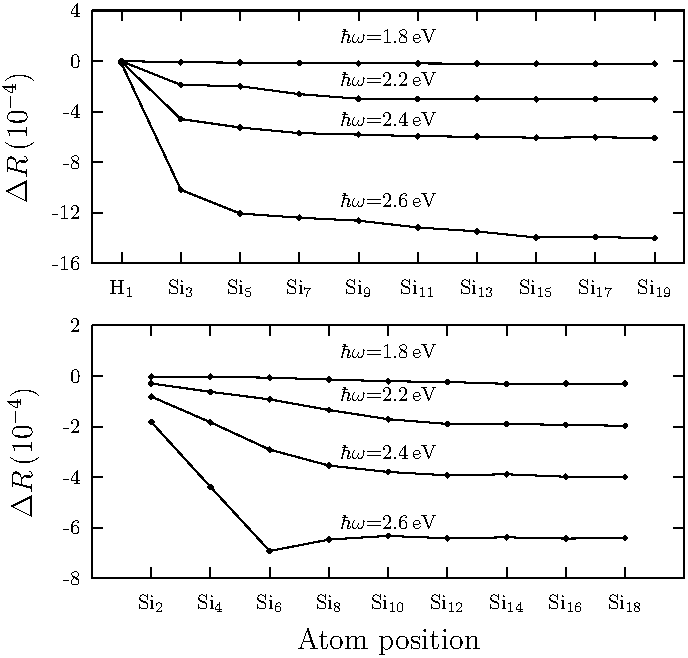
\includegraphics[width=0.9\linewidth]{fig04}
\caption{$\Delta R$ vs. the atom position for different values of $\hbar\omega$,
for atoms displaced \emph{down} by $p = 30\%$. Odd (H$_{1}$, Si$_{2n+1}$) atoms
are presented in the the top panel, and even (Si$_{2n}$) atoms in the bottom
panel. The solid lines are for ease of viewing.}
\label{fig:4}
\end{figure}

%%%%%%%%%%%%%%%%%%%%%%%%%%%%%%%%%%%%%%%%%%%%%%%%%%%%%%%%%%%%%%%%%%%%%%%%%%%%%%%
%%%%%%%%%%%%%%%%%%%%%%%%%%%%%%%%%%%%%%%%%%%%%%%%%%%%%%%%%%%%%%%%%%%%%%%%%%%%%%%

\section{Conclusions}\label{sec:conc}

We present a model to study the changes in reflectance induced by the
displacement of single atomic monolayers in a crystalline semiconductor slab,
and apply our model on the Si(111)(1$\times$1):H system. We find that the normal
incidence reflectance increases with respect to the relaxed system for
compressive and tensile strain, but only for incident photon energies above
$\sim2.0$\,eV. For our example system, we also found that most of the linear
optical response comes from elongated bonds, rather than from compressed ones.
The magnitude of our calculated results is within what is experimentally
measurable using lock-in techniques.

Although our scheme for displacing the atoms is a simplified depiction of a real
strain wave propagating through a material, it constitutes a first building
block for modeling more realistic systems. This model can be readily extended to
consider a superposition of displaced atomic layers, which would allow for
modeling different strain profiles. Our supercell method is also very flexible,
and can easily accommodate the inclusion of defects or deformities in the
crystalline lattice. 
{\color{red}Furthermore, a layer-by-layer analysis of the optical reflectance
can be readily studied within our current framework \cite{mendozaPRB06}.}
Ultimately, we consider that our \emph{ab initio} approach
is an attractive option for modeling the optoelectronic properties of a material
undergoing atomic disorder, and that extending our model could help understand
results from experimental techniques such as CAP spectroscopy or RAS.

%%%%%%%%%%%%%%%%%%%%%%%%%%%%%%%%%%%%%%%%%%%%%%%%%%%%%%%%%%%%%%%%%%%%%%%%%%%%%%%
%%%%%%%%%%%%%%%%%%%%%%%%%%%%%%%%%%%%%%%%%%%%%%%%%%%%%%%%%%%%%%%%%%%%%%%%%%%%%%%

\begin{acknowledgement}
We acknowledge useful discussions with {\color{red}N. Tolk} and Lucero Cano. Bernardo S.
Mendoza acknowledges partial support from CONACYT-M\'exico Grant 153930. Ram\'on
Carriles and Bernardo S. Mendoza thank the \emph{Red Nanociencias y
Nanotecnolog\'ia} of M\'exico for partial financial support.
\end{acknowledgement}

%%%%%%%%%%%%%%%%%%%%%%%%%%%%%%%%%%%%%%%%%%%%%%%%%%%%%%%%%%%%%%%%%%%%%%%%%%%%%%%
%%%%%%%%%%%%%%%%%%%%%%%%%%%%%%%%%%%%%%%%%%%%%%%%%%%%%%%%%%%%%%%%%%%%%%%%%%%%%%%

% \bibliography{refs}
\bibliographystyle{pss}

\providecommand{\WileyBibTextsc}{}
\let\textsc\WileyBibTextsc
\providecommand{\othercit}{}
\providecommand{\jr}[1]{#1}
\providecommand{\etal}{~et~al.}


\begin{thebibliography}{[10]}

\bibitem{hoganPRB98}% article
 \textsc{C.\,D. Hogan} and  \textsc{C.\,H. Patterson}\iffalse Reflectance
  anisotropy of silicon surfaces: {Discrete} dipole calculation\fi,
 \jr{Phys. Rev. B} \textbf{57}(23), 14843 (1998).


\bibitem{palummoPRB99}% article
 \textsc{M.~Palummo},  \textsc{G.~Onida},  \textsc{R.~Del~Sole},  and
  \textsc{B.\,S. Mendoza}\iffalse Ab initio optical properties of {Si}(100)\fi,
 \jr{Phys. Rev. B} \textbf{60}(4), 2522--2527 (1999).


\bibitem{hoganPRB03}% article
 \textsc{C.~Hogan},  \textsc{R.~Del~Sole},  and  \textsc{G.~Onida}\iffalse
  Optical properties of real surfaces from microscopic calculations of the
  dielectric function of finite atomic slabs\fi,
 \jr{Phys. Rev. B} \textbf{68}(3), 035405 (2003).


\bibitem{mendozaPRB06}% article
 \textsc{B.\,S. Mendoza},  \textsc{F.~Nastos},  \textsc{N.~Arzate},  and
  \textsc{J.~Sipe}\iffalse Layer-by-layer analysis of the linear optical
  response of clean and hydrogenated si(100) surfaces\fi,
 \jr{Phys. Rev. B} \textbf{74}(7), 075318 (2006).


\bibitem{palummoPRB09}% article
 \textsc{M.~Palummo},  \textsc{N.~Witkowski},  \textsc{O.~Pluchery},
  \textsc{R.~Del~Sole},  and  \textsc{Y.~Borensztein}\iffalse
  Reflectance-anisotropy spectroscopy and surface differential reflectance
  spectra at the {Si}(100) surface: {Combined} experimental and theoretical
  study\fi,
 \jr{Phys. Rev. B} \textbf{79}(3), 035327 (2009).


\bibitem{tancognePRB14}% article
 \textsc{N.~Tancogne-Dejean},  \textsc{B.\,S. Mendoza},  and
  \textsc{V.~V{\'e}niard}\iffalse Effect of material properties on the accuracy
  of antiresonant approximation: Linear and second-order optical responses\fi,
 \jr{Phys. Rev. B} \textbf{90}(3), 035212 (2014).


\bibitem{tancognePRB15}% article
 \textsc{N.~Tancogne-Dejean},  \textsc{C.~Giorgetti},  and
  \textsc{V.~V{\'e}niard}\iffalse Optical properties of surfaces with supercell
  {\emph{ab initio}} calculations: Local-field effects\fi,
 \jr{Phys. Rev. B} \textbf{92}(24), 245308 (2015).


\bibitem{thomsenPRL84}% article
 \textsc{C.\,H. Thomsen},  \textsc{J.~Strait},  \textsc{Z.~Vardeny},
  \textsc{H.\,J. Maris},  \textsc{J.~Tauc},  and  \textsc{J.\,J.
  Hauser}\iffalse Coherent phonon generation and detection by picosecond light
  pulses\fi,
 \jr{Phys. Rev. Lett.} \textbf{53}(10), 989 (1984).


\bibitem{thomsenPRB86}% article
 \textsc{C.\,H. Thomsen},  \textsc{H.\,T. Grahn},  \textsc{H.\,J. Maris},  and
  \textsc{J.~Tauc}\iffalse Surface generation and detection of phonons by
  picosecond light pulses\fi,
 \jr{Phys. Rev. B} \textbf{34}(6), 4129 (1986).


\bibitem{grahnJQE89}% article
 \textsc{H.\,T. Grahn},  \textsc{H.\,J. Maris},  and  \textsc{J.~Tauc}\iffalse
  Picosecond ultrasonics\fi,
 \jr{IEEE J. Quant. Electron.} \textbf{25}(12), 2562--2569 (1989).


\bibitem{linJAP91}% article
 \textsc{H.\,N. Lin},  \textsc{R.\,J. Stoner},  \textsc{H.\,J. Maris},  and
  \textsc{J.~Tauc}\iffalse Phonon attenuation and velocity measurements in
  transparent materials by picosecond acoustic interferometry\fi,
 \jr{J. Appl. Phys.} \textbf{69}(7), 3816--3822 (1991).


\bibitem{pfeiferPRL92}% article
 \textsc{T.~Pfeifer},  \textsc{W.~Kütt},  \textsc{H.~Kurz},  and
  \textsc{R.~Scholz}\iffalse Generation and detection of coherent optical
  phonons in germanium\fi,
 \jr{Phys. Rev. Lett.} \textbf{69}(22), 3248 (1992).


\bibitem{rossignolPRL05}% article
 \textsc{C.~Rossignol},  \textsc{J.\,M. Rampnoux},  \textsc{M.~Perton},
  \textsc{B.~Audoin},  and  \textsc{S.~Dilhaire}\iffalse Generation and
  detection of shear acoustic waves in metal submicrometric films with
  ultrashort laser pulses\fi,
 \jr{Phys. Rev. Lett.} \textbf{94}(16) (2005).


\bibitem{parkPRB05}% article
 \textsc{H.~Park},  \textsc{X.~Wang},  \textsc{S.~Nie},  \textsc{R.~Clinite},
  and  \textsc{J.~Cao}\iffalse Mechanism of coherent acoustic phonon generation
  under nonequilibrium conditions\fi,
 \jr{Phys. Rev. B} \textbf{72}(10) (2005).


\bibitem{wuAPL06}% article
 \textsc{S.~Wu},  \textsc{P.~Geiser},  \textsc{J.~Jun},  \textsc{J.~Karpinski},
   \textsc{J.\,R. Park},  and  \textsc{R.~Sobolewski}\iffalse Long-lived,
  coherent acoustic phonon oscillations in {GaN} single crystals\fi,
 \jr{Appl. Phys. Lett.} \textbf{88}(4), 041917 (2006).


\bibitem{matsudaPRL04}% article
 \textsc{O.~Matsuda},  \textsc{O.\,B. Wright},  \textsc{D.\,H. Hurley},
  \textsc{V.\,E. Gusev},  and  \textsc{K.~Shimizu}\iffalse Coherent {shear}
  {phonon} {generation} and {detection} with {ultrashort} {optical}
  {pulses}\fi,
 \jr{Phys. Rev. Lett.} \textbf{93}(9) (2004).


\bibitem{millerPRB06}% article
 \textsc{J.\,K. Miller},  \textsc{J.~Qi},  \textsc{Y.~Xu},  \textsc{Y.\,J.
  Cho},  \textsc{X.~Liu},  \textsc{J.\,K. Furdyna},  \textsc{I.~Perakis},
  \textsc{T.\,V. Shahbazyan},  and  \textsc{N.\,H. Tolk}\iffalse Near-bandgap
  wavelength dependence of long-lived traveling coherent longitudinal acoustic
  phonons in {GaSb}-{GaAs} heterostructures\fi,
 \jr{Phys. Rev. B} \textbf{74}(11) (2006).


\bibitem{wenAPL07}% article
 \textsc{Y.\,C. Wen},  \textsc{L.\,C. Chou},  \textsc{H.\,H. Lin},
  \textsc{V.~Gusev},  \textsc{K.\,H. Lin},  and  \textsc{C.\,K. Sun}\iffalse
  Efficient generation of coherent acoustic phonons in (111) {InGaAs}/{GaAs}
  multiple quantum wells through piezoelectric effects\fi,
 \jr{Appl. Phys. Lett.} \textbf{90}(17), 172102 (2007).


\bibitem{xuPSSC08}% article
 \textsc{Y.~Xu},  \textsc{J.~Qi},  \textsc{J.~Miller},  \textsc{Y.\,J. Cho},
  \textsc{X.~Liu},  \textsc{J.\,K. Furdyna},  \textsc{T.\,V. Shahbazyan},  and
  \textsc{N.\,H. Tolk}\iffalse Pump-probe studies of travelling coherent
  longitudinal acoustic phonon oscillations in {GaAs}\fi,
 \jr{physica status solidi (c)} \textbf{5}(8), 2632--2636 (2008).


\bibitem{babilottePRB10}% article
 \textsc{P.~Babilotte},  \textsc{P.~Ruello},  \textsc{D.~Mounier},
  \textsc{T.~Pezeril},  \textsc{G.~Vaudel},  \textsc{M.~Edely},  \textsc{J.\,M.
  Breteau},  \textsc{V.~Gusev},  and  \textsc{K.~Blary}\iffalse Femtosecond
  laser generation and detection of high-frequency acoustic phonons in {GaAs}
  semiconductors\fi,
 \jr{Phys. Rev. B} \textbf{81}(24) (2010).


\bibitem{hudertJAP08}% article
 \textsc{F.~Hudert},  \textsc{A.~Bartels},  \textsc{T.~Dekorsy},  and
  \textsc{K.~K{\"o}hler}\iffalse Influence of doping profiles on coherent
  acoustic phonon detection and generation in semiconductors\fi,
 \jr{J. Appl. Phys.} \textbf{104}(12), 123509 (2008).


\bibitem{limAPL03}% article
 \textsc{D.~Lim},  \textsc{R.\,D. Averitt},  \textsc{J.~Demsar},
  \textsc{A.\,J. Taylor},  \textsc{N.~Hur},  and  \textsc{S.\,W.
  Cheong}\iffalse Coherent acoustic phonons in hexagonal manganite {LuMnO}3\fi,
 \jr{Appl. Phys. Lett.} \textbf{83}(23), 4800--4802 (2003).


\bibitem{bozovicPRB04}% article
 \textsc{I.~Bozovic},  \textsc{M.~Schneider},  \textsc{Y.~Xu},
  \textsc{R.~Sobolewski},  \textsc{Y.\,H. Ren},  \textsc{G.~Lüpke},
  \textsc{J.~Demsar},  \textsc{A.\,J. Taylor},  and
  \textsc{M.~Onellion}\iffalse Long-lived coherent acoustic waves generated by
  femtosecond light pulses\fi,
 \jr{Phys. Rev. B} \textbf{69}(13) (2004).


\bibitem{ruelloPRB09}% article
 \textsc{P.~Ruello},  \textsc{S.~Zhang},  \textsc{P.~Laffez},
  \textsc{B.~Perrin},  and  \textsc{V.~Gusev}\iffalse Laser-induced coherent
  acoustical phonons mechanisms in the metal-insulator transition compound
  {NdNiO} 3 : {Thermal} and nonthermal processes\fi,
 \jr{Phys. Rev. B} \textbf{79}(9) (2009).


\bibitem{ruelloAPL12}% article
 \textsc{P.~Ruello},  \textsc{T.~Pezeril},  \textsc{S.~Avanesyan},
  \textsc{G.~Vaudel},  \textsc{V.~Gusev},  \textsc{I.\,C. Infante},  and
  \textsc{B.~Dkhil}\iffalse Photoexcitation of gigahertz longitudinal and shear
  acoustic waves in {BiFeO} $_{\textrm{3}}$ multiferroic single crystal\fi,
 \jr{Appl. Phys. Lett.} \textbf{100}(21), 212906 (2012).


\bibitem{chenAPL12}% article
 \textsc{L.\,Y. Chen},  \textsc{J.\,C. Yang},  \textsc{C.\,W. Luo},
  \textsc{C.\,W. Laing},  \textsc{K.\,H. Wu},  \textsc{J.\,Y. Lin},
  \textsc{T.\,M. Uen},  \textsc{J.\,Y. Juang},  \textsc{Y.\,H. Chu},  and
  \textsc{T.~Kobayashi}\iffalse Ultrafast photoinduced mechanical strain in
  epitaxial {BiFeO} $_{\textrm{3}}$ thin films\fi,
 \jr{Appl. Phys. Lett.} \textbf{101}(4), 041902 (2012).


\bibitem{gusevJAP11}% article
 \textsc{V.~Gusev},  \textsc{A.\,M. Lomonosov},  \textsc{P.~Ruello},
  \textsc{A.~Ayouch},  and  \textsc{G.~Vaudel}\iffalse Depth-profiling of
  elastic and optical inhomogeneities in transparent materials by picosecond
  ultrasonic interferometry: {Theory}\fi,
 \jr{J. Appl. Phys.} \textbf{110}(12), 124908 (2011).


\bibitem{matsudaJOSAB02}% article
 \textsc{O.~Matsuda} and  \textsc{O.\,B. Wright}\iffalse Reflection and
  transmission of light in multilayers perturbed by picosecond strain pulse
  propagation\fi,
 \jr{J. Opt. Soc. Am. B} \textbf{19}(12), 3028--3041 (2002).


\bibitem{grahnAPL88a}% article
 \textsc{H.\,T. Grahn},  \textsc{D.\,A. Young},  \textsc{H.\,J. Maris},
  \textsc{J.~Tauc},  \textsc{J.\,M. Hong},  and  \textsc{T.\,P. Smith}\iffalse
  Sound velocity and index of refraction of {AlAs} measured by picosecond
  ultrasonics\fi,
 \jr{Appl. Phys. Lett.} \textbf{53}(21), 2023--2024 (1988).


\bibitem{grahnAPL88b}% article
 \textsc{H.\,T. Grahn},  \textsc{H.\,J. Maris},  \textsc{J.~Tauc},  and
  \textsc{K.\,S. Hatton}\iffalse Elastic properties of silicon oxynitride films
  determined by picosecond acoustics\fi,
 \jr{Appl. Phys. Lett.} \textbf{53}(23), 2281--2283 (1988).


\bibitem{taneiPRL08}% article
 \textsc{H.~Tanei},  \textsc{N.~Nakamura},  \textsc{H.~Ogi},
  \textsc{M.~Hirao},  and  \textsc{R.~Ikeda}\iffalse Unusual elastic behavior
  of nanocrystalline diamond thin films\fi,
 \jr{Phys. Rev. Lett.} \textbf{100}(1) (2008).


\bibitem{qiPRB10}% article
 \textsc{J.~Qi},  \textsc{J.\,A. Yan},  \textsc{H.~Park},
  \textsc{A.~Steigerwald},  \textsc{Y.~Xu},  \textsc{S.\,N. Gilbert},
  \textsc{X.~Liu},  \textsc{J.\,K. Furdyna},  \textsc{S.\,T. Pantelides},  and
  \textsc{N.\,H. Tolk}\iffalse Mechanical and electronic properties of
  ferromagnetic {Ga$_{1-x}$Mn$_{x}$As} using ultrafast coherent acoustic
  phonons\fi,
 \jr{Phys. Rev. B} \textbf{81}(11) (2010).


\bibitem{zhuPRB91}% article
 \textsc{T.\,C. Zhu},  \textsc{H.\,J. Maris},  and  \textsc{J.~Tauc}\iffalse
  Attenuation of longitudinal-acoustic phonons in amorphous {SiO$_{2}$} at
  frequencies up to 440 {GHz}\fi,
 \jr{Phys. Rev. B} \textbf{44}(9), 4281 (1991).


\bibitem{dalyPRB09}% article
 \textsc{B.\,C. Daly},  \textsc{K.~Kang},  \textsc{Y.~Wang},  and
  \textsc{D.\,G. Cahill}\iffalse Picosecond ultrasonic measurements of
  attenuation of longitudinal acoustic phonons in silicon\fi,
 \jr{Phys. Rev. B} \textbf{80}(17) (2009).


\bibitem{tasAPL98}% article
 \textsc{G.~Tas},  \textsc{J.\,J. Loomis},  \textsc{H.\,J. Maris},
  \textsc{A.\,A. Bailes},  and  \textsc{L.\,E. Seiberling}\iffalse Picosecond
  ultrasonics study of the modification of interfacial bonding by ion
  implantation\fi,
 \jr{Appl. Phys. Lett.} \textbf{72}(18), 2235--2237 (1998).


\bibitem{steigerwaldJAP12}% article
 \textsc{A.~Steigerwald},  \textsc{A.\,B. Hmelo},  \textsc{K.~Varga},
  \textsc{L.\,C. Feldman},  and  \textsc{N.\,H. Tolk}\iffalse Determination of
  optical damage cross-sections and volumes surrounding ion bombardment tracks
  in {GaAs} using coherent acoustic phonon spectroscopy\fi,
 \jr{J. Appl. Phys.} \textbf{112}(1), 013514 (2012).


\bibitem{steigerwaldAPL09}% article
 \textsc{A.~Steigerwald},  \textsc{Y.~Xu},  \textsc{J.~Qi},
  \textsc{J.~Gregory},  \textsc{X.~Liu},  \textsc{J.\,K. Furdyna},
  \textsc{K.~Varga},  \textsc{A.\,B. Hmelo},  \textsc{G.~L{\"u}pke},
  \textsc{L.\,C. Feldman},  and  \textsc{N.\,H. Tolk}\iffalse Semiconductor
  point defect concentration profiles measured using coherent acoustic phonon
  waves\fi,
 \jr{Appl. Phys. Lett.} \textbf{94}(11), 111910 (2009).


\bibitem{gregoryAPL12}% article
 \textsc{J.~Gregory},  \textsc{A.~Steigerwald},  \textsc{H.~Takahashi},
  \textsc{A.~Hmelo},  and  \textsc{N.\,H. Tolk}\iffalse Ion implantation
  induced modification of optical properties in single-crystal diamond studied
  by coherent acoustic phonon spectroscopy\fi,
 \jr{Appl. Phys. Lett.} \textbf{101}(18), 181904 (2012).


\bibitem{baydinAPLP16}% article
 \textsc{A.~Baydin},  \textsc{H.~Krzyzanowska},  \textsc{M.~Dhanunjaya},
  \textsc{S.\,V.\,S. Nageswara~Rao},  \textsc{J.\,L. Davidson},  \textsc{L.\,C.
  Feldman},  and  \textsc{N.\,H. Tolk}\iffalse Depth dependent modification of
  optical constants arising from {H $^{\textrm{+}}$} implantation in n-type
  4h-{SiC} measured using coherent acoustic phonons\fi,
 \jr{APL Photonics} \textbf{1}(3), 036102 (2016).


\bibitem{mounierEPJST08}% article
 \textsc{D.~Mounier},  \textsc{E.~Morozov},  \textsc{P.~Ruello},
  \textsc{J.\,M. Breteau},  \textsc{P.~Picart},  and  \textsc{V.~Gusev}\iffalse
  Detection of shear picosecond acoustic pulses by transient femtosecond
  polarimetry\fi,
 \jr{Eur. Phys. J. Spec. Top.} \textbf{153}(1), 243--246 (2008).


\bibitem{mounierOE10}% article
 \textsc{D.~Mounier},  \textsc{P.~Picart},  \textsc{P.~Babilotte},
  \textsc{P.~Ruello},  \textsc{J.\,M. Breteau},  \textsc{T.~P{\'e}zeril},
  \textsc{G.~Vaudel},  \textsc{M.~Kouyat{\'e}},  and  \textsc{V.~Gusev}\iffalse
  Jones matrix formalism for the theory of picosecond shear acoustic pulse
  detection\fi,
 \jr{Opt. Express} \textbf{18}(7), 6767--6778 (2010).


\bibitem{lawlerMRE14}% article
 \textsc{H.\,M. Lawler},  \textsc{A.~Steigerwald},  \textsc{J.~Gregory},
  \textsc{H.~Krzyzanowska},  and  \textsc{N.\,H. Tolk}\iffalse Experimental and
  theoretical determination of the opto-acoustic spectrum of silicon\fi,
 \jr{Mater. Res. Express} \textbf{1}(2), 025701 (2014).


\bibitem{andersonPRB16b}% article
 \textsc{S.\,M. Anderson} and  \textsc{B.\,S. Mendoza}\iffalse Three-layer
  model for the surface second-harmonic generation yield including multiple
  reflections\fi,
 \jr{Physical Review B} \textbf{94}(11), 115314 (2016).


\bibitem{andersonFMATS17}% article
 \textsc{S.\,M. Anderson} and  \textsc{B.\,S. Mendoza}\iffalse Depth-dependent
  three-layer model for the surface second-harmonic generation yield\fi,
 \jr{Frontiers in Materials} \textbf{4}, 12 (2017).


\othercit
\bibitem{delsolechap95}% incollection
 \textsc{R.~Del~Sole},
Reflectance spectroscopy -- {T}heory,
 in: Photonic Probes of Surfaces, edited by P.~Halevi, No.~2 in Electromagnetic
  waves (Elsevier, Amsterdam; New York, 1995),  pp.\,131--174.


\bibitem{andersonPRB15}% article
 \textsc{S.\,M. Anderson},  \textsc{N.~Tancogne-Dejean},  \textsc{B.\,S.
  Mendoza},  and  \textsc{V.~V{\'e}niard}\iffalse Theory of surface
  second-harmonic generation for semiconductors including effects of nonlocal
  operators\fi,
 \jr{Phys. Rev. B} \textbf{91}(7), 075302 (2015).


\bibitem{gonzeCPS09}% article
 \textsc{X.~Gonze},  \textsc{B.~Amadon},  \textsc{P.\,M. Anglade},
  \textsc{J.\,M. Beuken},  \textsc{F.~Bottin},  \textsc{P.~Boulanger},
  \textsc{F.~Bruneval},  \textsc{D.~Caliste},  \textsc{R.~Caracas},
  \textsc{M.~C{\^{o}}t{\'{e}}},  \textsc{T.~Deutsch},  \textsc{L.~Genovese},
  \textsc{P.~Ghosez},  \textsc{M.~Giantomassi},  \textsc{S.~Goedecker},
  \textsc{D.\,R. Hamann},  \textsc{P.~Hermet},  \textsc{F.~Jollet},
  \textsc{G.~Jomard},  \textsc{S.~Leroux},  \textsc{M.~Mancini},
  \textsc{S.~Mazevet},  \textsc{M.\,J.\,T. Oliveira},  \textsc{G.~Onida},
  \textsc{Y.~Pouillon},  \textsc{T.~Rangel},  \textsc{G.\,M. Rignanese},
  \textsc{D.~Sangalli},  \textsc{R.~Shaltaf},  \textsc{M.~Torrent},
  \textsc{M.\,J. Verstraete},  \textsc{G.~Zerah},  and  \textsc{J.\,W.
  Zwanziger}\iffalse {ABINIT}: First-principles approach to material and
  nanosystem properties\fi,
 \jr{Comp. Phys. Commun.} \textbf{180}(12), 2582--2615 (2009).


\othercit
\bibitem{abinit}% misc
The ABINIT code is a common project of the Universit{\'e} Catholique de
  Louvain, Corning Incorporated, and other contributors (URL
  http://www.abinit.org).


\othercit
\bibitem{landolt}% book
 \textsc{H.~Landolt},  \textsc{R.~B{\"o}rnstein},  \textsc{K.\,H. Hellwege},
  \textsc{J.\,B. Goodenough},  \textsc{M.~Schulz},  \textsc{H.~Weiss},  and
  \textsc{O.~Madelung},
Numerical data and functional relationships in science and technology, New
  Series: Group III, Crystal and Solid State Physics,  Vol.\,17, Semiconductors
  (Springer, Berlin, 1984).


\bibitem{ortegaPRB93}% article
 \textsc{J.\,E. Ortega} and  \textsc{F.\,J. Himpsel}\iffalse
  Inverse-photoemission study of {Ge} (100), {Si} (100), and {GaAs} (100): Bulk
  bands and surface states\fi,
 \jr{Phys. Rev. B} \textbf{47}(4), 2130 (1993).


\bibitem{brunevalPRB06}% article
 \textsc{F.~Bruneval},  \textsc{N.~Vast},  and  \textsc{L.~Reining}\iffalse
  Effect of self-consistency on quasiparticles in solids\fi,
 \jr{Phys. Rev. B} \textbf{74}(4), 045102 (2006).


\bibitem{liPRB10}% article
 \textsc{Y.~Li} and  \textsc{G.~Galli}\iffalse Electronic and spectroscopic
  properties of the hydrogen-terminated {Si}(111) surface from ab initio
  calculations\fi,
 \jr{Phys. Rev. B} \textbf{82}(4), 045321 (2010).


\end{thebibliography}


\end{document}
